%&../settings/preamble.main

\ifsubfile
\pagestyle{plain}
\setcounter{chapter}{13}
\usepackage[
    parfill=30pt, % default: 30pt
]{parskip}

% arara: pdflatex: { options: ["--output-directory=../build"], draft: yes, synctex: no }
% arara: pdflatex: { options: ["--output-directory=../build"], synctex: no }
\begin{document}
\fi
\chapter{Scelta della struttura dati}

\begin{note}
La prima cosa da fare quando si progetta un algoritmo è capire quale sia la struttura dati adatta a risolvere quel particolare problema.
\end{note}

\section{Cammini minimi, sorgente singola}

\subsection{Problema dei cammini minimi}

\begin{definition}[Costo del cammino]
Dato un cammino \(p = \angleled{v_1, v_2, \ldots, v_k}\) con \(k > 1\), il \emph{costo del cammino} (\foreign{weight of the path}) è dato da
\begin{equation*}
w(p) = \sum_{i=2}^k w(v_{i-1}, v_i)
\end{equation*}
\end{definition}
Ossia dalla somma dei singoli pesi dei lati che compongono il percorso.

\paragraph{Definizione del problema}
Dati in input un grafo orientato \(G = (V, E)\), un nodo sorgente \(s\) ed una funzione di peso \(w \colon E \to R\) (che associa ad ogni arco un numero reale che rappresenta il peso).

Trovare un cammino da \(s\) ad \(u\), per ogni nodo \(u \in V\), il cui costo sia minimo, ovvero più piccolo o uguale al costo di qualunque altro cammino da \(s\) a \(u\).

\begin{note}
Non ci limitiamo a trovare un solo percorso, ma tutti i cammini da un nodo a tutti gli altri nodi.
\end{note}

\paragraph{Panoramica sul problema}

Per risolvere il problema del cammino minimo fra una coppia di vertici, si risolve il problema di cammini minimi da sorgente unica (si trovano tutti i cammini che partono da un nodo) e si estrae il cammino richiesto.
Per quanto riguarda il \emph{caso pessimo} non si conoscono algoritmi che abbiamo tempo di esecuzione migliore.

In alcuni casi gli archi possono avere peso negativo. Questo influisce sul problema (se è ben definito oppure no) e sulla soluzione (in assenza di archi negativi si \textcolor{red}{(possono?)} devono utilizzare tecniche diverse).

Nell'algoritmo di Dijkstra si suppone che tutti gli archi abbiano peso positivo, mentre nell'algoritmo di Bellman-Ford gli archi possono avere peso negativo, ma non possono esistere cicli di peso negativo.

\begin{note}
In generale possiamo ammettere pesi negativi, ma non cicli negativi.
\end{note}

\paragraph{Considerazioni sui cicli}
Se esiste un ciclo di peso negativo raggiungibile dalla sorgente, non esistono cammini finiti di peso minimo;
per qualunque cammino, basterà passare per un ciclo negativo più volte per ottenere un ciclo di costo inferiore.

Ovviamente, in un cammino minimo \emph{non è possibile la presenza di un ciclo di peso positivo}.
Mentre i cicli di peso nullo possono essere banalmente eliminati dal cammino minimo, in quanto inutili e ridondanti.

\subsection{Sottostruttura ottima}

Nota che due cammini minimi possono avere un tratto in comune, ma non possono convergere in un nodo comune \(B\) dopo aver percorso un tratto iniziale distinto.

\begin{figure}[H]\centering
	\begin{subfigure}[t]{.5\linewidth}\centering
		\includestandalone[mode=image]{walk-common-part}
		\caption{Due cammini minimi che hanno un tratto in comune a partire dal nodo \(B\)}%
		\label{fig:walk-common-part}
	\end{subfigure}%
	\begin{subfigure}[t]{.5\linewidth}\centering
		\includestandalone[mode=image]{walk-shared-node}
		\caption{Due cammini che convergono in un nodo comune \(B\) dopo aver percorso un tratto iniziale distinto.}%
		\label{fig:walk-shared-node}
	\end{subfigure}
	\caption{La figura~\ref{fig:walk-common-part} è una condizione ammissibile, mentre~\ref{fig:walk-shared-node} non lo è.}%
	\label{fig:sottostruttura-ottima}
\end{figure}

\begin{definition}[Albero dei cammini minimi]
L'albero dei cammini minimi è un albero di copertura radicato in \(s\) avente un cammino da \(s\) a tutti i nodi raggiungibili da \(s\).
\end{definition}

\begin{note}
Non confonderlo con gli alberi di copertura di peso minimo.
\end{note}

% NOTE è stato rimosso nelle nuove trasparenze?
\begin{definition}[Albero di copertura, \foreign{spanning tree}]
Dato un grafo \(G = (V, E)\) non orientato e connesso, un albero di copertura \(G\) è un sottografo di \(T = (V, E_T)\) tal che:
\begin{itemize}
	\item T è un albero;
	\item \(E_T \subseteq E\);
	\item \(T\) contiene tutti i vertici di \(G\).
\end{itemize}
\end{definition}

\paragraph{Soluzione ammissibile}
Una soluzione \emph{ammissibile} può essere descritta da un \emph{albero di copertura \(T\)} radicato in \(s\) e da un \emph{vettore delle distanze \(d\)}, i cui valori \(d[u]\) rappresentano il costo del cammino da \(s\) a \(u\) in \(T\).

\begin{figure}[H]\centering
	\begin{subfigure}[b]{.5\linewidth}\centering
		\includestandalone[mode=image]{shortestPath-admittable}
		\caption{Soluzione ammissibile (albero di peso minimo)}%
		\label{fig:soluzione-ammissibile}
	\end{subfigure}%
	\begin{subfigure}[b]{.5\linewidth}\centering
		\includestandalone[mode=image]{shortestPath-optimal}
		\caption{Soluzione ottima (albero dei cammini minimi)}%
		\label{fig:soluzione-ottima}
	\end{subfigure}
	\caption[Differenza fra albero di peso minimo e albero dei cammini minimi]
	        {Nota la differenza fra i due alberi: a sinistra l'albero di \emph{peso minimo} che rappresenta una soluzione ammissibile, ma non ottima, mentre a destra l'albero dei cammini minimi, ossia l'insieme dei percorsi che minimizzano il peso fra il nodo sorgente e tutti gli altri nodi, il quale rappresenta la soluzione ottima.}
\end{figure}

\begin{note}
In questo problema devo trovare i percorsi che minimizzano il peso fra un nodo e tutti gli altri nodi, e \textbf{non}, come sembra spontaneo fare, l'albero che ha complessivamente peso minimo.
\end{note}

\paragraph{Rappresentazione dell'albero}
Utilizziamo la rappresentazione basata su vettore dei padri, così come abbiamo fatto con le visite in ampiezza/profondità.

\subsection{Teorema di Bellman}

\begin{theorem}[Teorema di Bellman]
Una soluzione ammissibile \(T\) è (anche) ottima se e solo se:
\begin{align*}
d[v] \bs{=} d[u] + w (u,v)			& \text{ per ogni arco }(u,v) \bs{\in T} \\
d[v] \bs{\leqslant} d[u] + w (u,v)	& \text{ per ogni arco }(u,v) \bs{\in E}
\end{align*}
\end{theorem}
\begin{proof}[Dimostrazione per assurdo (parte 1)]
Sia \(T\) una soluzione ottima.
Consideriamo un qualunque arco \((u,v) \in E\) e sia \(w (u, w)\) la sua lunghezza.

Ovviamente se \((u,v) \in T\), allora \(d[v] = d[u] + w(u,v)\).
Invece se \((u,v) \notin T\), allora poiché \(T\) è ottimo, deve risultare \(d[v] \leqslant d[u] + w(u,v)\), altrimenti esisterebbe nel grafo \(G\) un cammino da \(s\) a \(v\) più corto di quello in \(T\), che è \emph{assurdo} perché abbiamo ipotizzato che \(T\) fosse ottima.
\end{proof}

\begin{proof}[Dimostrazione per assurdo (parte 2)]
Supponiamo per assurdo che il cammino da \(s\) a \(u\) in \(T\) non sia ottimo.
Allora esiste un cammino da \(s\) a \(u\) con distanza \(d'[u]<d[u]\).
Sia \(d'[v]\) la distanza da \(s\) ad un generico nodo \(v\) che appare in tale cammino.
Poichè \(d'[s] = d[s] = 0\), ma \(d'[u]<d[u]\), esiste un arco \((h,k)\) per cui \(d'[h] \geqslant d'[h]\) e \(d'[k]< d[k]\).
Per costruzione \(d_h' + w(h,k) = d_k'\).
Per ipotesi \(d_h + w(h,k) \ge d_k\).
Combinando queste due relazioni, si ottiene:
\begin{equation*}
d_k' = d_h' + w(h,k) \geqslant d_h + w(h,k) \geqslant d_k
\end{equation*}
che contraddice l'ipotesi.
\end{proof}

\subsection{Verso un algoritmo}

\begin{algorithm}[H]
	\caption{Algoritmo prototipo per il calcolo dei cammini minimi}
	%&../preamble

% arara: pdflatex: { synctex: no }
% arara: latexmk: { clean: partial }
\ifstandalone
\begin{document}
\begin{algorithm}[H]
\fi

\tcp{Algoritmo prototipo dei cammini minimi}
(\Int, \Int)\prototype{ \CamminiMinimi{\Graph \(G\), \Node \(s\)}}{

	\BlankLine
	\tcp{Inizializza \(T\) ad una foresta di copertura composta da nodi isolati}
	\tcp{Inizializza \(d\) con una sovrastima della distanza (\(d[s] = 0\), \(d[x] = +\infty\))}

	\BlankLine
	\While{\( \exists (u,v) \colon d[u] + G.\weight{u,v} < d[v] \)}{
		\tcp{Esiste un arco che mi permette di migliorare la stima}

		\BlankLine
		\(d[v] = d[u] + \weight{u,v}\) \Comment*[h]{Aggiorno la distanza}\;
		\tcp{Sostituisci il padre di \(v\) in \(T\) con \(u\)}
	}
	\Return \((T,d)\)
}

\ifstandalone
\end{algorithm}
\end{document}
\fi

\end{algorithm}

\paragraph{Commento}
L'algoritmo prende in input un grafo e il nodo sorgente.
I pesi vengono estratti dalla struttura dati \Graph.
Inizializziamo \(d\) con una sovrastima della distanza; \(d[s] = 0\) sta a significare che la sorgente ha distanza da sè stessa pari a 0 (caso base) e con \(d[x] = +\infty\) indico che la distanza di tutti gli altri nodi, fintanto che non è nota, è pari a \(+\infty\).

\begin{note}
Se al termine dell'esecuzione dell'algoritmo qualche nodo mantiene una distanza infinita, allora esso non è raggiungibile dalla sorgente.
\end{note}

\begin{algorithm}[H]
	\caption{Algoritmo generico per il calcolo dei cammini minimi}
	%&../preamble

% arara: pdflatex: { synctex: no }
% arara: latexmk: { clean: partial }
\ifstandalone
\begin{document}
\begin{algorithm}[H]
\fi

(\Int, \Int)\prototype{ \CamminiMinimi{\Graph \(G\), \Node \(s\)}}{

	\BlankLine
	\tcp{Inizializzazione dei vettori}
	\Array{\Int} \(d\) \Assign \new \Array{\Int}[1][G.n]
	\Comment*[r]{distanze dalla sorgente}

	\Array{\Int} \(T\) \Assign \new \Array{\Int}[1][G.n]
	\Comment*[r]{vettore dei padri}

	\Array{\Bool} \(b\) \Assign \new \Array{\Bool}[1][G.n]
	\Comment*[r]{per sapere in tempo costante se \(u \in S\)}

	\BlankLine
	\tcp{Inizializzo tutti i nodi tranne la sorgente}
	\ForEach{\(u \in G.\VV - \{s\}\)}{
		\(T[u] \Assign \Nil\) \Comment*[l]{non hanno padri}
		\(d[u] \Assign +\infty\) \Comment*[l]{non li ho ancora raggiunti}
		\(b[u] \Assign \False\) \Comment*[l]{non appartengono ancora all'insieme}
	}

	\BlankLine
	\tcp{Inizializzo la sorgente}
	\(T[s] \Assign \Nil\) \Comment*[h]{non ha padre}\;
	\(d[s] \Assign 0\) \Comment*[h]{per convenzione}\;
	\(b[s] \Assign \True\) \Comment*[h]{appartiene all'insieme}\;

	\BlankLine
	\lnl{shortestPath:init}%
	\alert{\DataStructure \(S \Assign \dsConstructor\)}\;
	\alert{\(S\).\dsAdd{s}}\;

	\BlankLine
	\While{\Not \(S.\setEmpty\)}{

		\lnl{shortestPath:remove}%
		\alert{\Int \(u \Assign S.\extract\)} \Comment*[l]{estraggo un nodo}
		\Array{b}{u} \Assign \False \Comment*[l]{non è più contenuto nella struttura dati}

		\BlankLine
		\ForEach(\Comment*[h]{per tutti i vicini}){\(v \in G.\adj(u)\)}{

			\BlankLine
			\If(\Comment*[h]{se migliora la stima}){\(d[u] + G.\weight{u,v} < d[v]\)}{
				% NOTE eIf incompatibile con l'opzione 'onelanguage'
				% NOTE in realtà è la traduzione sbagliata di "Else" in "allora"
				\eIf(\Comment*[h]{se non fa già parte dell'insieme}){\Not \(b[v]\)}{
					\lnl{shortestPath:add}%
					\alert{\(S.\dsAdd(v)\)} \Comment*[h]{aggiungilo}\;
					\(b[v] \Assign \True\) \Comment*[h]{fa parte dell'insieme}\;
				}{
					\lnl{shortestPath:shortest-update}%
					\alert{\footnotesize\ttfamily// Azione da intraprendere nel caso \(v\) sia già presente in \(S\)}
				}

				\BlankLine
				\tcp{aggiorno i vettori}
				\(T[v] \Assign u\)\;
				\(d[v] \Assign d[u] + G.\weight{u,v}\)\;
			}
		}
	}

	\Return \((T,d)\)\;
}

\ifstandalone
\end{algorithm}
\end{document}
\fi

\end{algorithm}

\paragraph{Commento}
\Array{\Bool} ci permette di sapere in tempo costante se un certo nodo appartiene ad una struttura dati oppure no, non sarà necessario quando implementeremo realmente il codice.

\newpage
\section{Algoritmo di Dijkstra}

Il seguente algoritmo è stato sviluppato da Edsger W.\ Dijkstra nel 1956, pubblicato nel 1959.
Nella versione originale veniva utilizzato per trovare la distanza minima fra due nodi sfruttando il concetto di coda con priorità.
Tieni conto però che le code di priorità basate sugli heap binari sono state proposte nel '64, infatti l'algoritmo che di solito viene considerato di Dijkstra è in realtà la versione modificata di Johnson.

\paragraph{Implementazione}
L'algoritmo utilizza una coda con priorità basata su vettore.

\begin{algorithm}[H]
	\caption{Algoritmo di Dijkstra}
	\setcounter{AlgoLine}{0}
	%&../preamble

% arara: pdflatex: { synctex: no }
% arara: latexmk: { clean: partial }
\ifstandalone
\begin{document}
\begin{algorithm}[H]
\fi

(\Array{\Int}, \Array{\Int})\prototype{ \CamminiMinimi{\Graph \(G\), \Node \(s\)}}{

	\BlankLine
	\lnlset{dijkstra:init}{1}%
	\alert{ \Heap \(S\) \Assign \heapConstructor } \Comment*[l]{\(\Omicron(n) \cdot 1\)}
	\alert{ \(S\).\heapInsert{\(s\), \(0\)} }\;

	\BlankLine
	\While(\Comment*[h]{\(\Omicron(n)\)}){\Not \(S.\setEmpty\)}{

		\lnlset{dijkstra:remove}{2}%
		\tcp{\(\Omicron(n)\) vettore ordinato / \(\Omicron(\log n)\) heap binario}
		\alert{\Int \(u\) \Assign \(S\).\heapDeleteMin }\;
		\(b[u]\) \Assign \False\;

		\BlankLine
		\ForEach{\( v \in G.\adj{u} \)}{
			\If{\(d[u] + G.\weight{u,v} < d[v] \)}{

				\BlankLine
				\eIf{\Not \(b[v]\)}{
					\tcp{\(\Omicron(1) \cdot n\) vettore ordinato / \(\Omicron(\log n) \cdot n\) heap binario}
					\lnlset{dijkstra:add}{3}%
					\alert{ \(S.\heapInsert{\(v\), \(d[u] + G.\weight{u,v}\)}\)} \;
					\(b[v]\) \Assign \True\;
				}{
					\tcp{\(\Omicron(1) \cdot m\) vettore ordinato / \(\Omicron(\log n) \cdot m\) heap binario}
					\lnlset{dijkstra:update}{4}%
					\alert{ \(S\).\heapDecrease{\(v\), \(d[u] + G.\weight{u,v}\)} }\;
				}

				\BlankLine
				\tcp{aggiorno i vettori}
				\(T[v]\) \Assign \(u\)\;
				\(d[v]\) \Assign \(d[u] + G.\weight{u,v}\)\;
			}
		}
	}
	\Return \((T, d)\)\;
}

\ifstandalone
\end{algorithm}
\end{document}
\fi

\end{algorithm}

\paragraph{Analisi della complessità}
% \vspace{-15pt}

\begin{itemize}
	\item[\circled{\ref{dijkstra:init}}]
	Viene creato un vettore di dimensione \(n\).
	Ogni elemento \(u\)-esimo rappresenta il nodo \(u\).
	Le priorità (distanze) vengono inizializzate ad \(+\infty\).
	La priorità di \(s\) è posta uguale a \(0\).
	Per un costo di \(O(n)\);

	\item[\circled{\ref{dijkstra:remove}}]
	Si ricerca il minimo all'interno del vettore, una volta trovato si \enquote{cancella} la sua priorità.
	Per un costo complessivo di \(O(n)\) (viene svolto all'interno di un ciclo);

	\item[\circled{\ref{dijkstra:add}}]
	Si registra la priorità nella posizione corrispondente all'indice \(v\).
	Per un costo di \(O(1)\);

	\item[\circled{\ref{dijkstra:update}}]
	Si aggiorna la priorità nella posizione corrispondente all'indice \(v\).
	Per un costo di \(O(1)\).
\end{itemize}

% \vspace{-15pt}
\subsubsection*{Esempio di esecuzione}
% \vspace{-10pt}

\begin{minipage}[c]{0.5\textwidth}\centering
	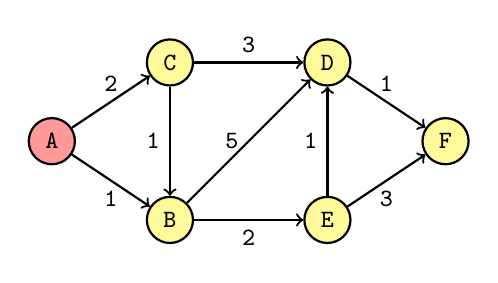
\begin{tikzpicture}[
	    thick,
	    font=\ttfamily\bfseries\small
	]
	\tikzset{
	    mynode/.style = {circle, draw=black, align=center,fill=yellow!40},
	    mynoder/.style = {circle, draw=black, align=center,fill=red!40},
	    edgen/.style = {->,thick},
	    edger/.style = {->,ultra thick,red}
	}
	\node[mynoder] at (0.0,1.0) (a) {A};
	\node[mynode]  at (1.5,0.0) (b) {B};
	\node[mynode]  at (1.5,2.0) (c) {C};
	\node[mynode]  at (3.5,2.0) (d) {D};
	\node[mynode]  at (3.5,0.0) (e) {E};
	\node[mynode]  at (5.0,1.0) (f) {F};
	\draw[edgen] (a) edge node[below] {1} (b);
	\draw[edgen] (a) edge node[above] {2} (c);
	\draw[edgen] (c) edge node[left] {1} (b);
	\draw[edgen] (c) edge node[above] {3} (d);
	\draw[edgen] (b) edge node[left] {5} (d);
	\draw[edgen] (b) edge node[below] {2} (e);
	\draw[edgen] (e) edge node[below] {3} (f);
	\draw[edgen] (e) edge node[left] {1} (d);
	\draw[edgen] (d) edge node[above] {1} (f);
	\end{tikzpicture}
\end{minipage}%
\begin{minipage}[c]{0.5\textwidth}\centering
	\begin{tabular}{@{} c ? *{7}{c} @{}}
		&&A&B&C&D&E&F \\
	\thickrule
		A & 0 & \textbf{0} & \(\cancel{0}\) & \(\cancel{0}\) & \(\cancel{0}\) & \(\cancel{0}\) & \(\cancel{0}\) \\
		B & \(\infty\) & 1 & \textbf{1} & \cancel{1} & \cancel{1} & \cancel{1} & \cancel{1} \\
		C & \(\infty\) & 2 & 2 & \textbf{2} & \cancel{2} & \cancel{2} & \cancel{2} \\
		D & \(\infty\) & \(\infty\) & 6 & 5 & 4 & \textbf{4} & 4\\
		E & \(\infty\) & \(\infty\) & 3 & 3 & \textbf{3} & \cancel{3} & \cancel{3} \\
		F & \(\infty\) & \(\infty\) & \(\infty\) & \(\infty\) & 6 & 5 & \textbf{5} \\
	\end{tabular}
\end{minipage}

\begin{itemize}
	\item ogni colonna contiene lo stato del vettore $d$ all'inizio di ogni ripetizione del ciclo \textsf{while} \Not S.\setEmpty
	\item ogni riga \(v\) rappresenta l'evoluzione dello stato dell'elemento \(d[v]\);
	\item la legenda delle colonne rappresenta il nodo che viene estratto.
\end{itemize}

\paragraph{Correttezza}
Tutte le volte che estraiamo un nodo, quel nodo ha una distanza (priorità) positiva ed estraiamo nodi a distanza progressivamente crescenti.
Se estraggo un nodo dalla coda tutti gli altri nodi hanno distanze più grandi.
Tutte le volte che estraggo un nodo la sua distanza non può più essere modificata.
Ed è questo il motivo per cui l'algoritmo di Dijkstra funziona (bene) solo con pesi positivi.

\begin{note}
L'algoritmo di Dijkstra funziona correttamente solo con pesi positivi.
\end{note}

\subsection{Correttezza per pesi positivi}

Ogni nodo viene estratto una e una sola volta.
Al momento dell'estrazione la sua distanza è minima.

\begin{proof}[Dimostrazione per induzione sul numero \(k\) di nodi estratti]
Per \(k=0\) (caso base) è vero poiché \mbox{\(d[s]=0\)} e non ci sono lunghezze negative.
Supponiamo che sia vero per i primi \(k-1\) nodi (ipotesi induttiva).
Quando viene estratto il \(k\)-esimo nodo \(u\), la sua distanza \(d[u]\) dipende dai \(k-1\) nodi già estratti (passo induttivo).
Non può quindi dipendere dai nodi ancora da estrarre, che hanno distanza \(\geqslant d[u]\).
Di conseguenza \(d[u]\) è minimo e \(u\) non verrà più re-inserito, perché non ci sono distanze negative.
\end{proof}

\section{Algoritmo di Johnson}

\paragraph{Analisi della complessità}
% \(\Omicron(n^2 + m)\) ma siccome \(m = \Omicron(n^2)\), allora il costo è \(\Omicron(n^2)\).
Con l'introduzione dell'heap binario nel '64 le operazioni che prima venivano svolte con complessità \(\Omicron(n)\) sul vettore ordinato ora hanno complessità \(\Omicron(\log n)\).
Di conseguenza la complessità totale dell'algoritmo scende da \(\Omicron(n^2)\) a \(\Omicron(m \log n)\).

Per \emph{grafi densi} non conviene utilizzare uno heap binario in quanto \(m = \Theta(n^2)\) e di conseguenza l'algoritmo avrebbe una complessità di \(\Omicron(n^2 \log n)\) si preferisce quindi la versione con vettore ordinato per una complessità di \(\Omicron(n^2)\), mentre per \emph{grafi sparsi} \(m = \Theta(n)\) e l'algoritmo \(\Omicron(n \log n)\) che è migliore di \(\Omicron(m \log n)\).

\section{Algoritmo di Fredman-Tarjan}

\paragraph{Analisi della complessità}
Sfruttando un heap di fibonacci l'operazione di \heapDecrease ha costo ammortizzato costante; così facendo hanno abbassato la complessità a \(\Omicron(m + n \log n)\).
Per \emph{grafi sparsi} produce un miglioramento nella complessità.

\newpage
\section{Algoritmo di Bellman-Ford-Moore}

\begin{note}
\'E computazionalmente più pesante dell'algoritmo di Dijkstra ma può lavorare anche con archi di peso negativo.
\end{note}

\paragraph{Implementazione}
Utilizza una coda senza priorità.

\begin{algorithm}[H]
	\caption{Algoritmo di Bellman-Ford-Moore}
	%&../preamble

% arara: pdflatex: { synctex: no }
% arara: latexmk: { clean: partial }
\ifstandalone
\begin{document}
\begin{algorithm}[H]
\fi

(\Array{\Int}, \Array{\Int})\prototype{\ \CamminiMinimi{\Graph \(G\), \Node \(s\)}}{

	\BlankLine
	\lnlset{bellman:init}{1}%
	\alert{ \Queue \(S\) \Assign \queueConstructor }\;
	\alert{ \(S.\queueInsert{s}\) } \Comment*[h]{metto in coda il nodo sorgente}\;

	\BlankLine
	\While(\Comment*[h]{\(\Omicron(n)\)}){\Not \(S\).\setEmpty}{

		\lnlset{bellman:remove}{2}%
		\alert{ \Int \(u\) \Assign \(S\).\queueRemove } \Comment*[l]{\(\Omicron(1 \cdot n)\)}
		\(b[u]\) \Assign \False\;

		\BlankLine
		\ForEach{\( v \in G.\adj{u} \)}{
			\If{\( d[u] + G.\weight{u,v} < d[v] \)}{

				\BlankLine
				\If{\Not \(b[v]\)}{
					\lnlset{bellman:add}{3}%
					\tcp{lo metto in cosa quando c'è un miglioramento}
					\alert{ \(S.\queueInsert{v}\) } \Comment*[h]{\(\Omicron(m \cdot n)\)}\;
					\(b[v]\) \Assign \True\;
				}
			}
		}
	}
	\Return \((T, d)\)\;
}

\ifstandalone
\end{algorithm}
\end{document}
\fi

\end{algorithm}

\begin{itemize}
	\item [\circled{\ref{bellman:init}}]
	Viene creata una coda di dimensione \(n\).
	Per un costo computazionale di \(O(n)\);
	\item [\circled{\ref{bellman:remove}}]
	Viene estratto il prossimo elemento della coda.
	Per un costo computazionale di \(O(1)\);
	\item [\circled{\ref{bellman:add}}]
	Si inserisce l'indice \(v\) in coda.
	Per un costo computazionale di \(O(1)\).
\end{itemize}

L'inserimento in coda può essere fatto più di una volta durante il ciclo di esecuzione dell'algoritmo, al contrario di quel che accade nell'algoritmo di Dijkstra.
Il passo \circled{4} non è necessario in quanto non c'è una priorità da aggiornare.

\subsubsection*{Esempio di esecuzione}

\begin{minipage}[c]{0.5\textwidth}\centering
	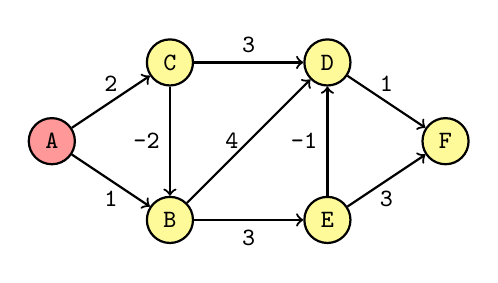
\begin{tikzpicture}[
	    thick,
	    font=\ttfamily\bfseries\small
	]
	\tikzset{
	    mynode/.style = {circle, draw=black, align=center,fill=yellow!40},
	    mynoder/.style = {circle, draw=black, align=center,fill=red!40},
	    edgen/.style = {->,thick},
	    edger/.style = {->,ultra thick,red}
	}
		\node[mynoder] at (0.0,1.0) (a) {A};
		\node[mynode]  at (1.5,0.0) (b) {B};
		\node[mynode]  at (1.5,2.0) (c) {C};
		\node[mynode]  at (3.5,2.0) (d) {D};
		\node[mynode]  at (3.5,0.0) (e) {E};
		\node[mynode]  at (5.0,1.0) (f) {F};
		\draw[edgen] (a) edge node[below] {1} (b);
		\draw[edgen] (a) edge node[above] {2} (c);
		\draw[edgen] (c) edge node[left] {-2} (b);
		\draw[edgen] (c) edge node[above] {3} (d);
		\draw[edgen] (b) edge node[left] {4} (d);
		\draw[edgen] (b) edge node[below] {3} (e);
		\draw[edgen] (e) edge node[below] {3} (f);
		\draw[edgen] (e) edge node[left] {-1} (d);
		\draw[edgen] (d) edge node[above] {1} (f);
	\end{tikzpicture}
\end{minipage}%
\begin{minipage}[c]{0.5\textwidth}
\paragraph{Come leggere la tabella sottostante}
\begin{itemize}[leftmargin=*]
	\item la prima riga contiene l'elemento estratto dalla coda;
	\item l'ultima riga contiene lo stato della coda;
	\item i vettori delle distanze sono rappresentate dalle colonne.
\end{itemize}
\end{minipage}

\begin{table}[H]\centering
	\begin{tabu}{ r @{\hskip 5pt} >{\ttfamily\small}c ? c | c  | cc | ccc | ccc | c | c @{\hskip 5pt}}
		\rowfont{\ttfamily\small}
			nodo estratto:& & & A & B & C & D & E & B & F & D & E & D & F \\
		\Xcline{2-14}{1pt}
			\multirow[c]{6}{*}{\rotatebox[origin=c]{90}{vettori}}
						   & A & 0 & 0 & 0 & 0 & 0 & 0 & 0 & 0 & 0 & 0 & 0 & 0 \\
						   & B & \(\infty\) & 1 & 1 & 0 & 0 & 0 & 0 & 0 & 0 & 0 & 0 & 0 \\
						   & C & \(\infty\) & 2 & 2 & 2 & 2 & 2 & 2 & 2 & 2 & 2 & 2 & 2 \\
						   & D & \(\infty\) & 5 & 5 & 5 & 3 & 3 & 3 & 3 & 3 & 2 & 2 & 2 \\
						   & E & \(\infty\) & \(\infty\) & 4 & 4 & 4 & 4 & 3 & 3 & 3 & 3 & 3 & 3 \\
						   & F & \(\infty\) & \(\infty\) & \(\infty\) & \(\infty\) & 6 & 5 & 5 & 5 & 4 & 4 & 3 & 3 \\
		\Xcline{2-14}{1pt}\rowfont{\ttfamily\small}
	 			queue:& S & A & BC & CDE & DEB & EBF & BFD & FDE & DE & E & D & F & \\
	\end{tabu}
\end{table}

\paragraph{Dimostrazione di correttezza}
Per dimostrare la correttezza dell'algoritmo dobbiamo dare la definizione di \enquote{passata}.
Una passata si definisce ricorsivamente come segue: per \(k = 0\), la zeresima passata consiste nell'estrazione del nodo \(s\) dalla coda \(S\), per \(k > 0\) la \(k\)-esima passata consiste nell'estrazione di tutti i nodi presenti in \(S\) al termine della passata \(k-1\)-esima.
Viene data solo un'intuizione, non viene fatta una dimostrazione formale.
Al termine della passata \(k\), i vettori \(T\) e \(d\) descrivono i cammini minimi di lunghezza al più \(k\).
Al termine della passata \(n-1\), i vettori \(T\) e \(d\) descrivono i cammini (di lunghezza al più \(n-1\)).

\paragraph{Analisi della complessità}
L'inserimento in coda dei nodi avviene solo una volta per un costo di \(\Omicron(1)\).
Un nodo può essere estratto e reinserito al massimo \(n-1\) volte, per un costo di \(\Omicron(n^2)\).
Quando avviene un miglioramento la distanza viene aggiornata, per un costo i \(\Omicron(n \dot m)\).
Il costo complessivo dell'algoritmo risulta quindi \(\Omicron(n \dot m)\).

\paragraph{Cammini minimi su DAG}
I cammini minimi su DAG sono sempre ben definiti;
anche in presenza di pesi negativi, in quanto non esistono cicli (nè tantomeno quelli negativi).
\'E possibile rilassare gli archi \emph{in ordine topologico}, \emph{una volta sola}.
Non essendoci cicli, non c'è modo di tornare su un nodo già visitato ed abbassare il valore della sua distanza (il suo campo \(d\)).

Si utilizza quindi l'ordine topologico.

\begin{algorithm}[H]
	\caption{Algoritmo di Bellman-Ford-Moore applicato su DAG}
	%&../preamble

% arara: pdflatex: { synctex: no }
% arara: latexmk: { clean: partial }
\ifstandalone
\begin{document}
\begin{algorithm}[H]
\fi

(\Array{\Int}, \Array{\Int})\prototype{\ \CamminiMinimi{\Graph \(G\), \Node \(s\)}}{

	\BlankLine
	\Array{\Int} \(d =\) \new \Array{\Int}[1][G.n] \Comment*[r]{\(d[u]\) è la distanza da \(s\) a \(u\)}
	\Array{\Int} \(T =\) \new \Array{\Int}[1][G.n] \Comment*[r]{\(T[u]\) è il padre da \(u\) nell'albero \(T\)}

	\BlankLine
	\tcp{Inizializzo i vettori}
	\ForEach{\(u \in G.\VV - \{s\}\)}{
		\(T[u] = \Nil\)\;
		\(d[u] = +\infty\)\;
	}

	\BlankLine
	\tcp{Inizializzo la sorgente}
	\(T[s] = \Nil\)\;
	\(d[u] = 0\)\;

	\BlankLine
	\tcp{Effettuo l'ordinamento topologico dei nodi nel DAG}
	\Stack \(S = \topSort\)\;

	\BlankLine
	\tcp{fintanto che la pila non è vuota}
	\While{\Not \(S.\setEmpty\)}{
		\(u = S.\stackPop\) \tcp{estraggo un nodo}
		\ForEach(\tcp*[h]{per ogni nodo adiacente}){\(v \in G.\adj{v}\)}{
			\If(\tcp*[h]{se il peso è migliore di quello presente}){\(d[u] + G.\weight{u,v} < d[v]\)}{

				\BlankLine
				\tcp{aggiorno il peso}
				\(T[v] = u\)\;
				\(d[v] = d[u] + G.\weight{u,v}\)\;
			}
		}
	}

	\BlankLine
	\tcp{restituisco il vettore dei padri e il vettore delle distanze}
	\Return (\(T\), \(d\))\;
}

\ifstandalone
\end{algorithm}
\end{document}
\fi

\end{algorithm}

\newpage
\subsection{Riassumendo}

\begin{table}[H]\centering
\caption{Quale complessità preferire?}%
\label{tab:complexity-compared}
\begin{tabularx}{\textwidth}{@{} *{4}{l} @{}}
	\toprule
		\textbf{Algoritmo} & \textbf{Complessità} & \textbf{Input}\\
	\midrule
		Dijkstra		& \(\Omicron(n^2)\)				& Pesi positivi, grafi denso  \\
	\lightrule
		Johnson			& \(\Omicron(m \log n)\)		& Pesi positivi, grafi sparso \\
	\lightrule
		Fredman-Tarjan	& \(\Omicron(m + n \log n)\)	& Pesi positivi, grafi denso, dimensioni molto grandi \\
	\lightrule
		Bellman-Ford	& \(\Omicron(m \cdot n)\)		& Pesi negativi \\
						& \(\Omicron(m + n)\)			& DAG			\\
					\lightrule
		BFS				& \(\Omicron(m + n)\)			& Senza pesi	\\
	\bottomrule
\end{tabularx}
\end{table}

\subsection{Cammini minimi, sorgente multipla}

Vogliamo cercare i cammini minimi fra tutti i nodi.

\begin{table}[!ht]
\caption{Quale complessità preferire?}%
\label{tab:complexity-compared}
\begin{tabularx}{\textwidth}{@{} *{3}{l} @{}}
	\toprule
	\textbf{Algoritmo} & \textbf{Complessità} & \textbf{Input}\\
	\midrule
	Pesi positivi, grafo denso & \(\Omicron(n \cdot n^2)\) & Applicazione ripetuta (\(n\)) dell'algoritmo di Dijkstra \\
	\lightrule
	Pesi positivi, grafo sparso & \(O(n \cdot (m \log n))\) & Applicazione ripetuta dell'algoritmo di Johnson \\
	\lightrule
	Pesi negativi & \(O(n \cdot nm)\) & Applicazione ripetuta di Bellman-Ford (sconsigliata) \\
	\lightrule
	Pesi negativi, grafo denso & \(O(n^3)\) & Algoritmo di \textbf{Floyd e Warshall} \\
	\lightrule
	Pesi negativi, grafo sparso & \(O(nm \log n)\) & Algoritmo di \textbf{Johnson per sorgente multipla}\\
	\bottomrule
\end{tabularx}
\end{table}

L'algoritmo di Bellman-Ford è sconsigliato per grafi densi perché può arrivare ad avere una complessità di \(\Omicron(n^4)\), mentre l'algoritmo di Floyd e Warshall ha una complessità di \(\Omicron(n^3)\) indipendentemente dalla forma del grafo.

\newpage
\section{Algoritmo di Floyd-Warshall}

Utilizza la programmazione dinamica.
Ci riesce ridefinendo la definione del costo di cammino in modo tale che possa essere calcolato in modo ricorsivo.

\begin{definition}[Cammini minimi \(k\)-vincolati]
Sia \(k\) un valore in \(\{0, \dots, n\}\).
Diciamo che un cammino \(p_{xy}^{k}\) è un cammino minimo \(k\)-vincolato fra \(x\) ed \(y\) se esso ha il costo minimo fra tutti i cammini fra \(x\) e \(y\) che non passano per nessun vertice in \(v_{k+1}, \dots, v_n\) (\(x\) e \(y\) sono esclusi dal vincolo).
\end{definition}

\begin{note}
Assumiamo, come abbiamo sempre fatto, che esista un ordinamento fra i nodi del grafo \(v_1, v_2, \dots, v_n\).
\end{note}

% \(p_{xy}^{0}\) corrisponde a
% \(p_{xy}^{n}\) corrisponde a

\begin{definition}[Distanza \(k\)-vincolata]
Denotiamo con \(d^{k}[x][y]\) il costo totale del cammino minimo \(k\)-vincolato fra \(x\) e \(y\), se esiste.
\[
d^{k}[x][y] =
	\begin{dcases}
		w(p_{xy}^{k}) & \text{se esiste }p_{xy}^{k}\\
		+\infty & \text{altrimenti}\\
	\end{dcases}
\]
\end{definition}

% \(d^{0}[x][y]\) corrisponde a
% \(d^{n}[x][y]\) corrisponde a

La formulazione ricorsiva è la seguente:
\[
d^{k}[x][y] =
	\begin{dcases}
		d[x][y] & k = 0\\
		d^{k-1}[x][y] \lor d^{k-1}[x][k] \land d^{k-1}[k][y] & k > 0\\
	\end{dcases}
\]
Ad esempio:

% TODO esternare le immagini
\begin{minipage}[c]{0.5\textwidth}\centering
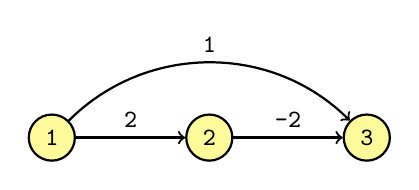
\begin{tikzpicture}[
    thick,
    font=\ttfamily\bfseries\small
]
	\tikzset{
	    mynode/.style = {circle, draw=black, align=center,fill=yellow!40},
	    mynoder/.style = {circle, draw=black, align=center,fill=red!40},
	    edgen/.style = {->,thick},
	    edger/.style = {->,ultra thick,red}
	}
	\node[mynode] at (0.0,0.0) (a) {1};
	\node[mynode] at (2.0,0.0) (b) {2};
	\node[mynode] at (4.0,0.0) (c) {3};
	\draw[edgen] (a) edge node[above] {2} (b);
	\draw[edgen] (b) edge node[above] {-2} (c);
	\draw[edgen] (a) edge[bend left=45] node[above] {1} (c);
\end{tikzpicture}
\end{minipage}%
\begin{minipage}[c]{0.5\textwidth}\centering
\begin{align*}
d^{0}[1][3] &= 1 \\
d^{1}[1][3] &= 1 \\
d^{2}[1][3] &= \minFunction(d^{1}[1][3], d^{1}[1][2] + d^{2}[2][3]) \\
			&= \minFunction(1, +2-2) \\
			&= \minFunction(1, 0) = 0 \\
\end{align*}
\end{minipage}

% TODO [39-40]

Oltre a definire la matrice \(d\), calcoliamo una matrice \(T\) dove \(T[x][y]\) rappresenta il predecessore di \(y\) nel cammino più breve da \(x\) a \(y\).
Ad esempio:

\begin{minipage}[c]{0.5\textwidth}\centering
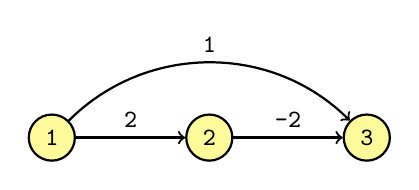
\begin{tikzpicture}[
    thick,
    font=\ttfamily\bfseries\small
]
	\tikzset{
	    mynode/.style = {circle, draw=black, align=center,fill=yellow!40},
	    mynoder/.style = {circle, draw=black, align=center,fill=red!40},
	    edgen/.style = {->,thick},
	    edger/.style = {->,ultra thick,red}
	}
	\node[mynode] at (0.0,0.0) (a) {1};
	\node[mynode] at (2.0,0.0) (b) {2};
	\node[mynode] at (4.0,0.0) (c) {3};
	\draw[edgen] (a) edge node[above] {2} (b);
	\draw[edgen] (b) edge node[above] {-2} (c);
	\draw[edgen] (a) edge[bend left=45] node[above] {1} (c);
\end{tikzpicture}
\end{minipage}%
\begin{minipage}[c]{0.5\textwidth}\centering
\begin{align*}
T[1][2] &= 1 \\
T[2][3] &= 2 \\
T[1][3] &= 2 \\
\end{align*}
\end{minipage}

% TODO scrivere l'algoritmo
\begin{algorithm}[H]
	\caption{Algoritmo di Floyd-Warshall}
	%&../preamble

% arara: pdflatex: { synctex: no }
% arara: latexmk: { clean: partial }
\ifstandalone
\begin{document}
\begin{algorithm}[H]
\fi

(\Array{\Int}, \Array{\Int})\prototype{\ \CamminiMinimi{\Graph \(G\), \Node \(s\)}}{

	\BlankLine
	\tcp{Credo le matrici}
	\Matrix{\Int} \(d =\) \new \Matrix{\Int}[1\dots n][1\dots n] \Comment*[r]{matriche delle distanze}
	\Matrix{\Int} \(T =\) \new \Matrix{\Int}[1\dots n][1\dots n] \Comment*[r]{matriche dei padri (predecessori)}

	\BlankLine
	\tcp{Inizializzo i vettori}
	\ForEach{\(u, v \in G.\VV\)}{
		\(d[u][v] = +\infty\)\;
		\(T[u][v] = \Nil\)\;
	}

	\BlankLine
	\tcp{Inserisco i valori iniziali}
	\ForEach{\(u \in G.\VV\)}{
		\ForEach{\(v \in G.\adj{u}\)}{
			\(d[u][v] = G.\weight(u, v)\)\;
			\(T[u][v] = u\)\;
		}
	}

	\BlankLine
	\tcp{Aggiorno le distanze}
	\From{\(k \Assign 1\) \DownTo \(G.n\)}{
		\ForEach{\(u \in G.\VV\)}{
			\ForEach{\(v \in G.\adj{u}\)}{
				\If{\( d[u][k] + d[k][v] < d[u][v] \)}{
					\(d[u][v] = d[u][k] + d[k][v]\)\;
					\(T[u][v] =T[k][v]\)\;
				}
			}
		}
	}

	\BlankLine
	\Return \(d\)\;
}

\ifstandalone
\end{algorithm}
\end{document}
\fi

\end{algorithm}

\section{Algoritmo di Warshall}

\begin{definition}[Chiusura transitiva]
La chiusura transitiva \(G^* = (V, E^*)\) di un grafo \(G = (V, E)\) è il grafo orientato tale che \((u, v) \in E^*\) se e solo esiste un cammino da \(u\) a \(v\) in \(G\).
\end{definition}

Supponendo di avere il grafo \(G\) rappresentato da una matrice di adiacenza \(M\), la matrice \(M^n\) rappresenta la matrice di adiacenza di \(G^*\).

La formulazione ricorsiva è la seguente:
\[
M^{k}[x][y] =
	\begin{dcases}
		M[x][y] & k = 0\\
		M^{k-1}[x][y] \lor M^{k-1}[x][k] \land M^{k-1}[k][y] & k > 0\\
	\end{dcases}
\]

\section*{Conclusioni}

Abbiamo visto una panoramica dei più importanti algoritmi per la ricerca dei cammini minimi.
Esistono anche altri algoritmi, in particolare l'algortimo \(A^*\) utilizza euristiche per velocizzare la ricerca.

\ifsubfile
\end{document}
\fi
